%\documentclass[a4paper,bibtotoc,oneside]{scrbook}	%für lange Arbeiten: Chapter ist die höchste Ebene
\documentclass[a4paper,bibtotoc,oneside]{scrartcl}	%für kurze Arbeiten: Section ist die höchste Ebene
\usepackage[utf8]{inputenc}
\usepackage[T1]{fontenc}
\usepackage{lmodern}
\usepackage[ngerman]{babel}
\usepackage{listings}
\usepackage{float}


% verlinkte Querverweise im pdf
\usepackage{hyperref}		% immer als letztes laden

% mathematische Symbole
\usepackage{amsmath,amssymb,amsfonts,amstext}

% Kopfzeilen frei gestaltbar
\usepackage{fancyhdr}
\lfoot[\fancyplain{}{}]{\fancyplain{}{}}
\rfoot[\fancyplain{}{}]{\fancyplain{}{}}
\cfoot[\fancyplain{}{\footnotesize\thepage}]{\fancyplain{}{\footnotesize\thepage}}
\lhead[\fancyplain{}{\footnotesize\nouppercase\leftmark}]{\fancyplain{}{}}
\chead{}
\rhead[\fancyplain{}{}]{\fancyplain{}{\footnotesize\nouppercase\sc\leftmark}}

% Farben im Dokument m"oglich
\usepackage{color}

% Schriftart Helvetica
\usepackage{helvet}
\renewcommand{\familydefault}{cmss}

% Graphiken einbinden: hier f"ur pdflatex
\usepackage[pdftex]{graphicx}
\usepackage{pdfpages}

\usepackage{array}

% H"ohe und Breite des Textk"orpers etwas gr"osser definieren
\setlength{\textheight}{225mm}
\setlength{\textwidth}{1.05\textwidth}

% weniger Warnungen wegen "uberf"ullter Boxen
\tolerance = 9999
\sloppy

% Anpassung einiger "Uberschriften
\renewcommand\figurename{Abbildung}
\renewcommand\tablename{Tabelle}
\begin{document}

% Kopf- und Fusszeilen initiieren
\pagestyle{fancy}

% Deckblatt:
\thispagestyle{empty}
\begin{picture}(0,0)
	\color{white}\sffamily
	\put(-101,-412){
\includegraphics[width=1.002\paperwidth]{LPS_2011.pdf}}
	\put(220,-670){
\includegraphics[width=0.5\textwidth]{FHTW_Logo_4c.pdf}}
	\put(-30, -20){\bfseries\huge Software Requirements Specification}

	% Titel der Lehrveranstaltung einf"ugen:
	\put(-30,-70){\Large Lehrveranstaltung IT Projektarbeit}
	\color{black}
	% Titel der Arbeit einf"ugen:
	% Die Minipage wird gesetzt, damit auch mehrzeilige Titel m"oglich werden.
	\put(-32,-350){
		\begin{minipage}{13cm}
			\bfseries\huge Polaroid Fotoclub Webseite 
		\end{minipage}
	}
	% Name der Autorin/des Autors eingeben:
	\put(-30,-450){\large Ausgeführt von: David Wolf, Leonhardt Schwarz, Tom Schalbar, Christoph Müllner}
	% Personenkennzeichen der Autorin/des Autors eingeben:
	%\put(-30,-470){\large Personenkennzeichen: if12b076}
	% Name der Begutachterin/des Begutachters eingeben:
	\put(-30,-510){\large Begutachter: Veronika Winter}
	\put(-30,-550){\large Wien, \today} % das Datum des letzten Kompilierens wird automatisch eingesetzt
\end{picture}


\newpage
\begin{table}[h]
	\centering
	\begin{tabular}{|c|l|l|}
		\hline
		\textbf{Version} & \textbf{Datum} & \textbf{Change} \\
		\hline
		0.1.0 & 2014/02/28 & Erste Erstellung des Dokuments \\
		\hline
		0.1.1 & 2014/03/19 & ERD \& Mockups wurden hinzugefügt \\
		\hline
	\end{tabular}

	\caption{Dokumentenentwicklung}
	\label{tab:Dokumentenentwicklung}
\end{table}

\newpage
\tableofcontents\thispagestyle{empty}
\newpage
\setcounter{page}{1}

% Falls die Kapitel"uberschriften zu lang f"ur die Kopfzeile oder das Inhaltsverzeichnis sind, so erzielt man
% dort Kurzformen der Kapitelbezeichnungen mittels:
% \chapter[Kurzform]{Lange "Uberschrift}

\section{Vision und Kurzbeschreibung des Projekts}
	Eine responsive Webseite zum Anzeigen und Archivieren von Fotos soll 
	mit modernen Webtechnologien realisiert werden.
	\paragraph{Ziel:}
		Implementation einer Webseite welche sowohl auf Desktop PCs als
		auch auf Mobiltelefonen in kontinuierlichem Design angezeigt
		wird. Ein Nutzer soll einen Account anlegen können und Fotos auf
		die Webseite hochladen können. Andere Nutzer sollen dann in der
		Lage sein diese Fotos zu bewerten und kommentieren zu können.
		Um die Privatsphäre des Nutzers zu wahren können mithilfe einer
		Freundeverwaltung Fotos nur bestimmten Nutzern zugänglich 
		gemacht werden.

\section{Überblick über die geforderte Funktionalität}
	\begin{itemize}
		\item Anlegen und verwalten von Accounts
		\item Hochladen von Fotos
		\item Responsive/ Fluid Design
		\item Albumverwaltung
		\item Fotos bewerten, kommentieren und gegebenenfalls dem
		Administrator melden
		\item Administratorbereich
		\item Statistiken zu hochgeladenen Fotos (Viewcount)
		\item Freundeverwaltung
		\item Einstellungen zur Privatsphäre (Nur Freunde können
		bestimmte Fotos sehen)
		\item Suchfilter
	\end{itemize}
\section{Systemabgrenzung und detaillierte Funktionale Anforderungen}
	\subsection{Node.js}
	Node.js ist eine serverseitige Plattform zum Betrieb von
	Netzwerkanwendungen.  Insbesondere lassen sich Webserver damit 
	realisieren.  Node.js basiert auf der JavaScript-Laufzeitumgebung „V8“,
	die ursprünglich für den Chrome-Browser entwickelt wurde und bietet 
	daher eine ressourcensparende Architektur, die eine besonders große
	Anzahl gleichzeitig bestehender Netzwerkverbindungen ermöglicht

\section{Schnittstellen}
	\subsection{Benutzerschnittstellen}
		\subsubsection{Webseite}
			\begin{figure}[H]
			\centering
				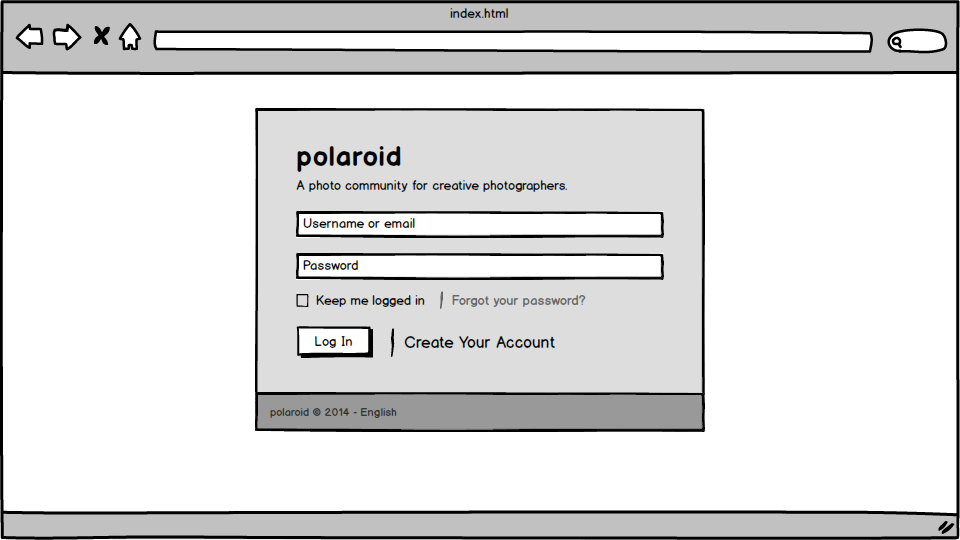
\includegraphics[width=400px]{Mockups/01_login.jpeg}
				\caption{Mockup: Login} 
				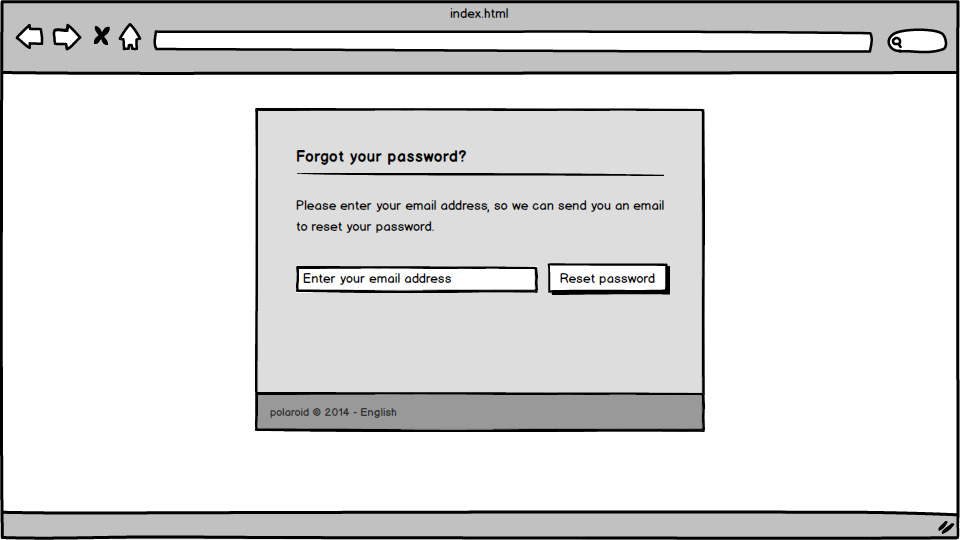
\includegraphics[width=400px]{Mockups/02_password.jpeg}
				\caption{Mockup: Forgot your password}
			\end{figure}
			\begin{figure}[H]
				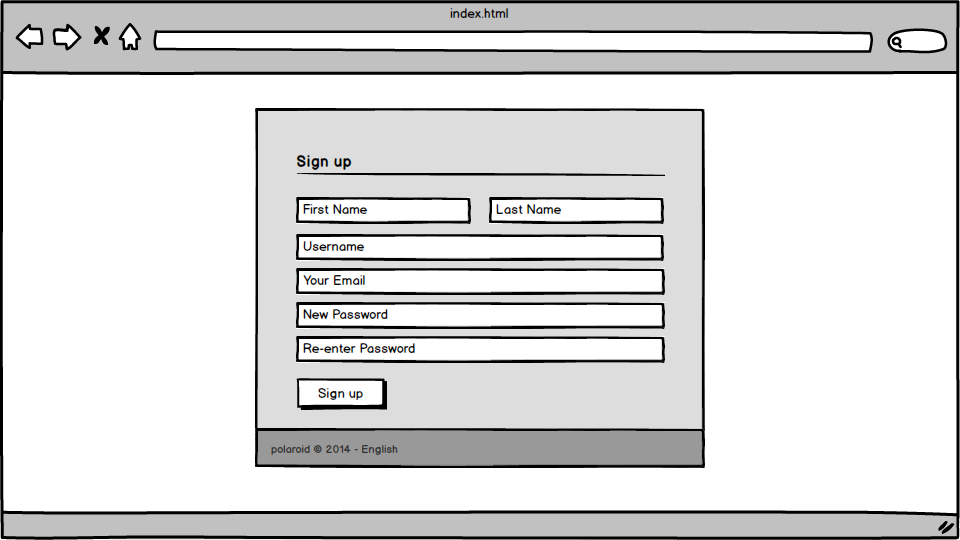
\includegraphics[width=400px]{Mockups/03_signup.jpeg}
				\caption{Mockup: Registrierungsformular}
				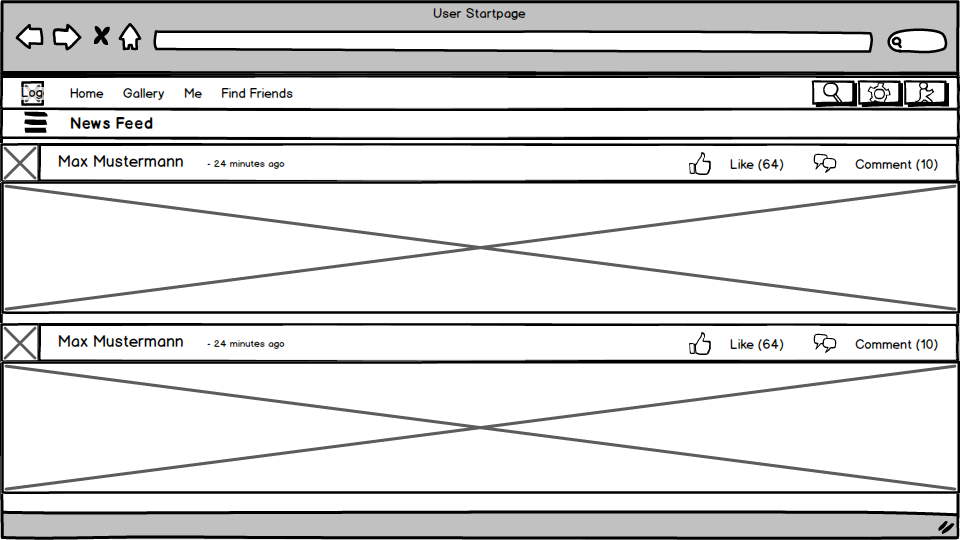
\includegraphics[width=400px]{Mockups/04_startpage.jpeg}
				\caption{Mockup: News Feed - Seite}
			\end{figure}
			\begin{figure}[H]
				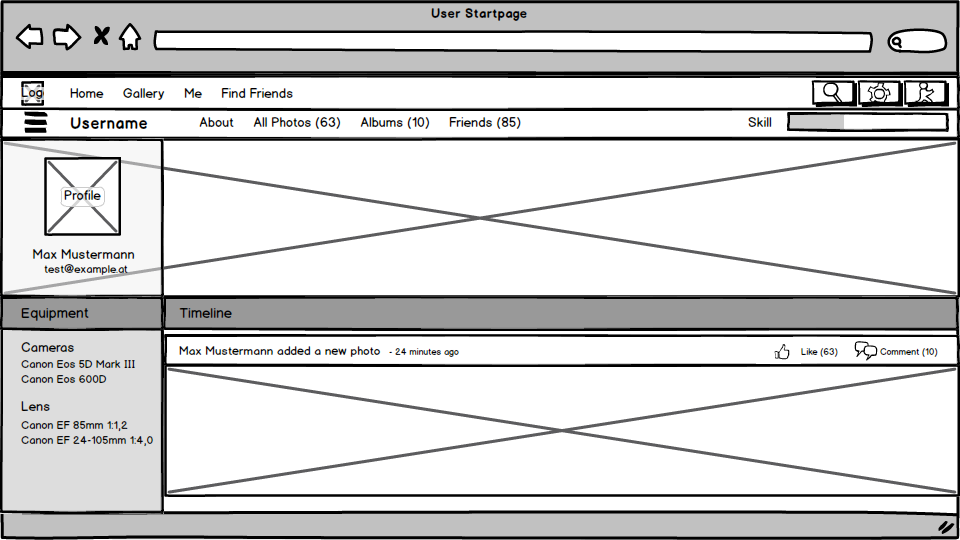
\includegraphics[width=400px]{Mockups/05_profile.jpeg}
				\caption{Mockup: Profil - Seite}
				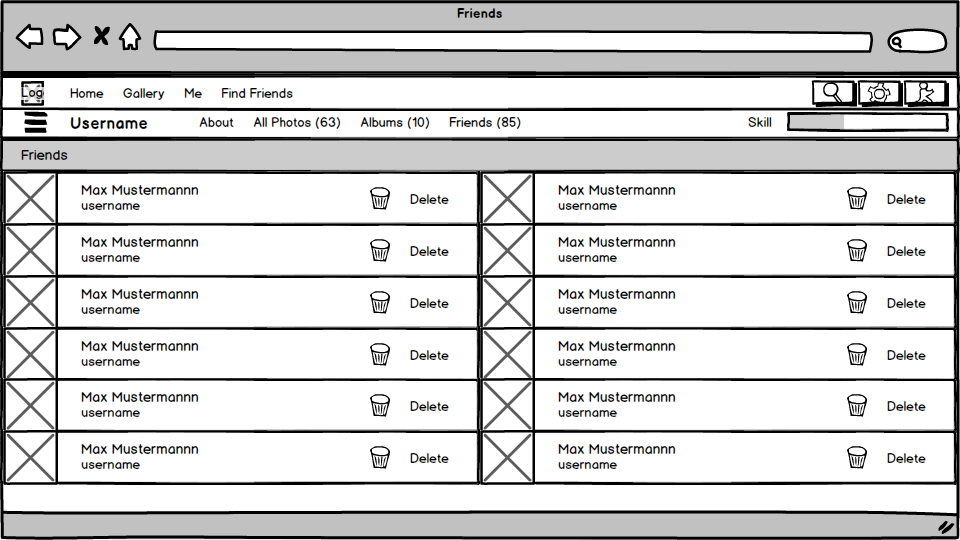
\includegraphics[width=400px]{Mockups/06_friends.jpeg}
				\caption{Mockup: Meine Freunde - Seite}
			\end{figure}
			\begin{figure}[H]
				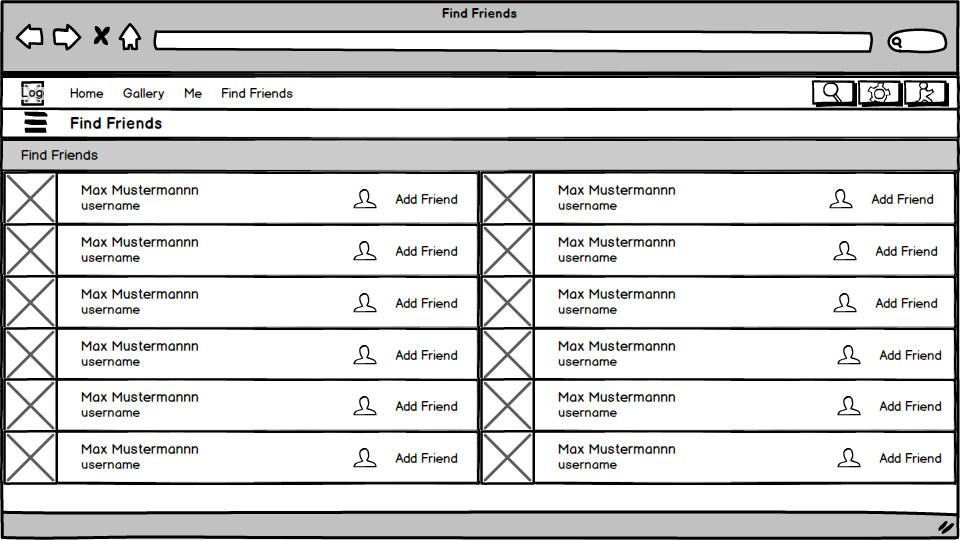
\includegraphics[width=400px]{Mockups/07_find_friends.jpeg}
				\caption{Mockup: Suche nach Freunde}
				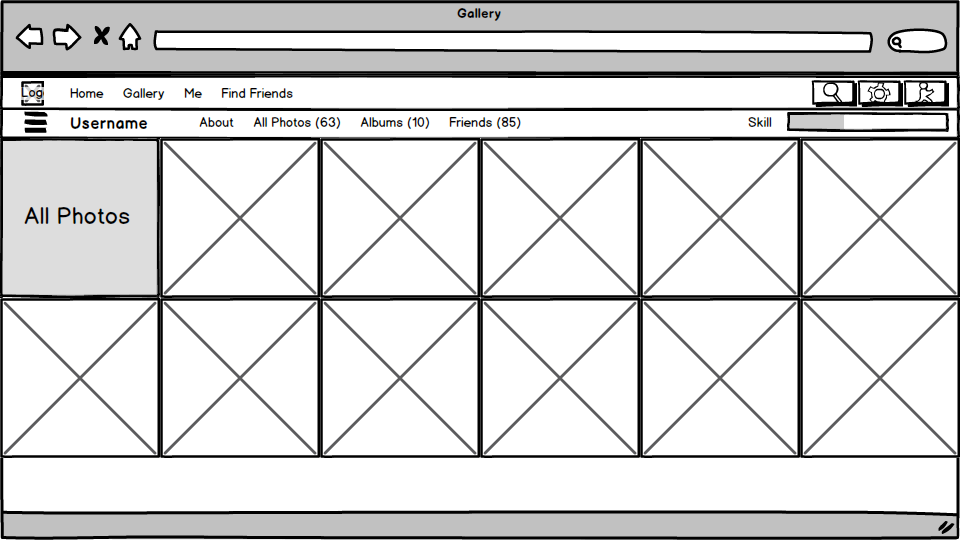
\includegraphics[width=400px]{Mockups/08_user_gallery.jpeg}
				\caption{Mockup: Galerieansicht}
			\end{figure}
			\begin{figure}[H]
				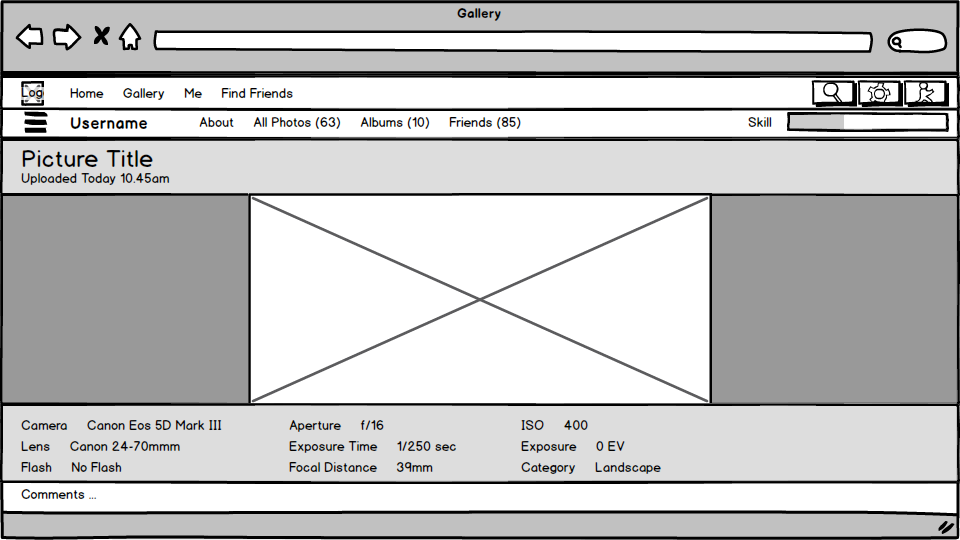
\includegraphics[width=400px]{Mockups/09_user_gallery_photo.jpeg}
				\caption{Mockup: Foto-Ansicht}
				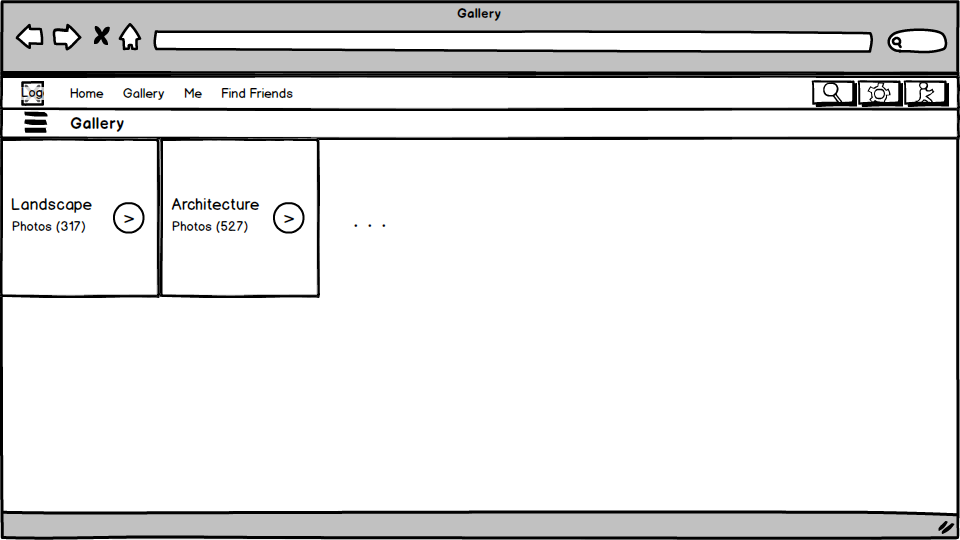
\includegraphics[width=400px]{Mockups/10_gallery_cat.jpeg}
				\caption{Mockup: Galerie Kategorie}
			\end{figure}
			\begin{figure}[H]
				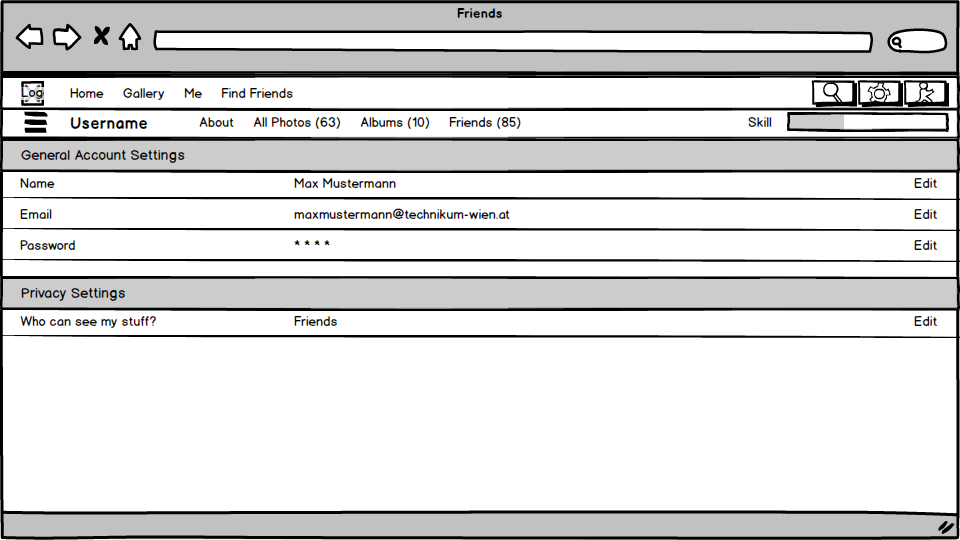
\includegraphics[width=400px]{Mockups/11_setting.jpeg}
				\caption{Mockup: Einstellungen}
			\end{figure}
	\subsection{Systemschnittstellen}
		\subsubsection{Webseite}
		\subsubsection{Webserver}
			Der Webserver kommuniziert über Expressjs mit dem Client. Zuerst wird der Port angebunden und dann werden alle Requests an Expressjs weitergeleitet. Expressjs sendet dann den Verarbeiteten Request an das Routingmodul. Das Routingmodul hat wiederum eine Anbindung mit dem DB-Modul. Das DB-Modul kapselt dann schließlich die Datenbank zugriffe.\\
			
			\noindent Expressjs selber hat zusätzlich noch einiges an Middleware die hier kurz zusammengefasst werden soll.
			
			\paragraph{connect-multiparty}
			Dient dazu Form-Requests die mit dem \textit{enctype} 'multipart/form-data' gesendet werden, auch erfolgreich zu verarbeiten. Im wensentlichen wird der gesendet Body verarbeitet und in einem JSON Objekt gekapselt über den Request gesendet.
			
			\paragraph{body-parser}
			Dieses Middleware dient der Vorverarbeitung von Request-Bodies. Dazu wird der gesendete Body des Clients in ein JSON Objekt gekapselt. Um jedoch Binärdaten übertragen zu können, muss das zuvor erwähnte connect-multiparty Middleware dazu installiert werden.
			
			\paragraph{cookie-parser}
			Dieses Middleware dient dazu die vom Client gesendeten Cookies in ein einfach zu lesendes Array zu laden.
			
			\paragraph{cookie-session}
			Dieses Middleware erlaubt es Signed-Cookies zu übertragen und zu interpretieren.
			
			\paragraph{express-session}
			Einfach gesagt erlaubt dieses Middleware die Manipulation von der Client-Session. Hierfür wird eine eigene Sessionvariable angelegt die man beliebig ändern kann.
			
			\paragraph{Session}
			Es werden zum Teil wichtige Variablen in die Session gespeichert. Lesen kann man sie durch den Request mit der folgenden Syntax '\textit{request.session.$<$variable$>$}'. Nachfolgend werden die existierenden Variablen samt Bedeutung beschrieben:
			
			\begin{center}
			\begin{tabular}{|l|l|}
			\hline
			\bf Variable & \bf Bedeutung \\
			\hline
			username & Speichert den Anwendernamen. \\
			\hline
			\end{tabular}
			\end{center}
			
			\paragraph{Schnittstellen}
			\begin{center}
			\begin{tabular}{|lcr|}
			\hline
			Nodejs & $\Leftrightarrow$ & Expressjs \\
			\hline
			Expressjs & $\Leftrightarrow$ & Middleware \\
			\hline
			Expressjs & $\Leftrightarrow$ & Routing \\
			\hline
			Routing & $\Leftrightarrow$ & DB \\
			\hline
			DB & $\Leftrightarrow$ & Datenbank \\
			\hline
			\end{tabular}
			\end{center}
			
		\subsubsection{Datenbank}

			\begin{figure}[H]
			\centering
			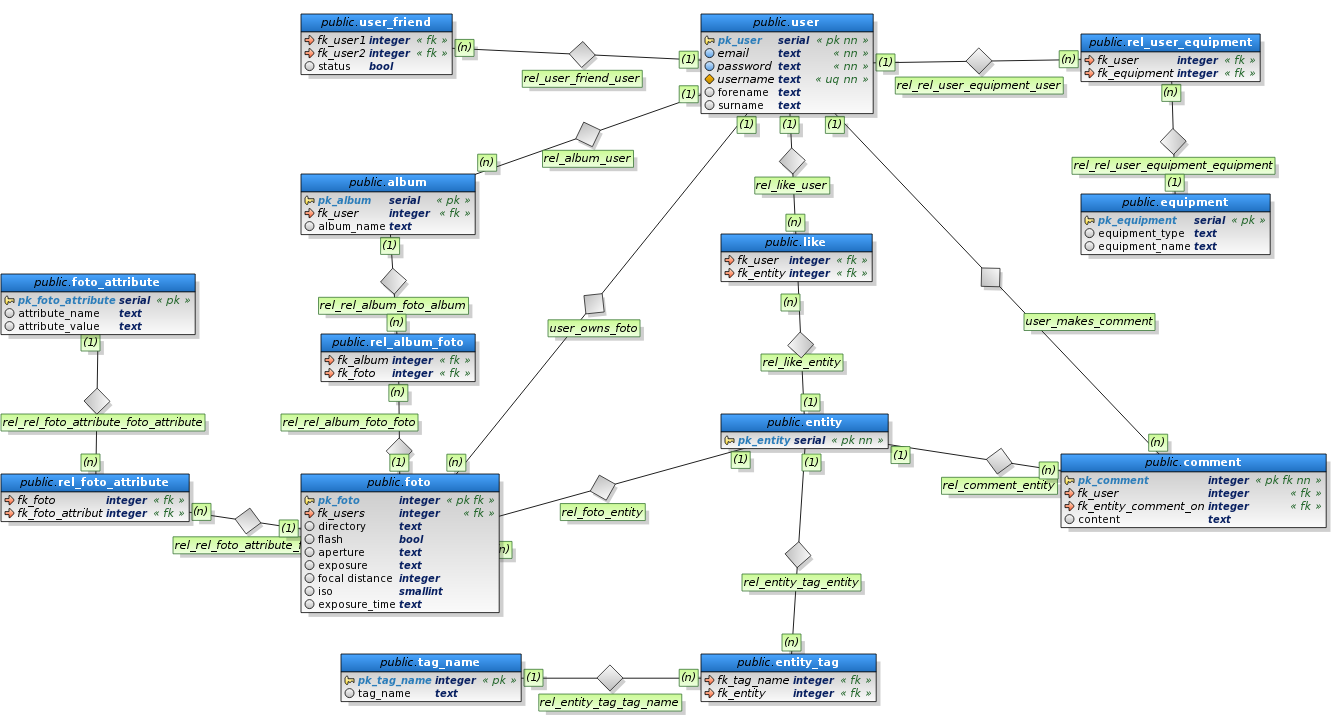
\includegraphics[width=400px]{Mockups/db_v1.png}
			\caption{Datenbank: ERD}
			\end{figure}

\section{Nicht-Funktionale Anforderungen}
	\subsection{Vorgaben zu Hardware und Software}
		\subsubsection{Software}
			\begin{itemize}
				\item OpenSSL >= 1.0.1g
				\item Postgres >= 9.3
				\item Node.js >= 0.10.27
				\item ImageMagick >= 6.8.9-2
				\item PostgreSQL
				\item Ein moderner Browser welcher HTML5 \& CSS3 unterstützt
			\end{itemize}
		
			\noindent Die benötigten Module von Nodejs werden durch die \textit{package.json} definiert.
			Für eine Installation reicht das Kommando \textit{npm install} in dem Verzeichnis mit
			der \textit{package.json}.
			
		\subsubsection{IP Forwarding}
			Es gibt zwei Server, einen HTTP-Server und einen HTTPS-Server. Der HTTP-Server bindet
			sich an den Port 8080, von daher ist es notwendig sämtlichen IP-Traffic vom Port 80
			zum Port 80 weiterzuleiten.\\
			
			\noindent Der HTTP-Server dient der Weiterleitung von HTTP-Requests zu HTTPS-Requests.
			Der eigentliche Datenverkehr findet mit HTTPS statt. Hierfür muss dann der IP-Traffic
			von Port 443 auf den Port 43443 weitergeleitet werden.
	\subsection{Usability}

\section{Rahmenbedingungen}
\subsection{Meilsteine}
	\begin{itemize}
		\item 1. Meilenstein: Login, Registrierung, Passwort vergessen fertigstellen (Frotend \& Backend), 10 April 2014

	\end{itemize}
\subsection{Übersicht}
	\begin{itemize}
		\item Entwicklungsumgebung Windows 8/Linux/OS X
		\item Javascript
		\item HTML5 \& CSS3
		\item Node.js
		\item PostgreSQL
	\end{itemize}

\section{Lieferumfang}
	\begin{itemize}
		\item Dokumentation
		\item Webseite
	\end{itemize}
\newpage
\listoffigures
\addcontentsline{toc}{section}{List of figures}
\bibliographystyle{abbrv}
\bibliography{main}

\end{document}
